\section{Theorem von Nyquist}

Im Folgenden soll das Theorem von Nyquist genauer betrachtet werden. Dafür wird der Ausgang des Frequenzgenerator direkt mit dem Eingang des Messcomputers verbunden, parallel dazu wird der Ausgang des Generators mit dem Osziloskop überprüft.\\
Das Theorem besagt das ein Signal, begrenzt mit $f_{max}$, nur mit einer Abtastfrequenz von größer $f_{crit}$ exakt rekonstruiert werden kann.
\begin{align}
    f_{crit} = 2 \cdot f_{max}
\end{align}


Um dies genauer zu untersuchen wurde zuerst die Abtastrate für ein unverrauschtes Sinussignal ($f = 20$\,kHz) variiert und gegen die gemessene Frequenz aufgetragen.
\begin{figure}[h]
    \centering
    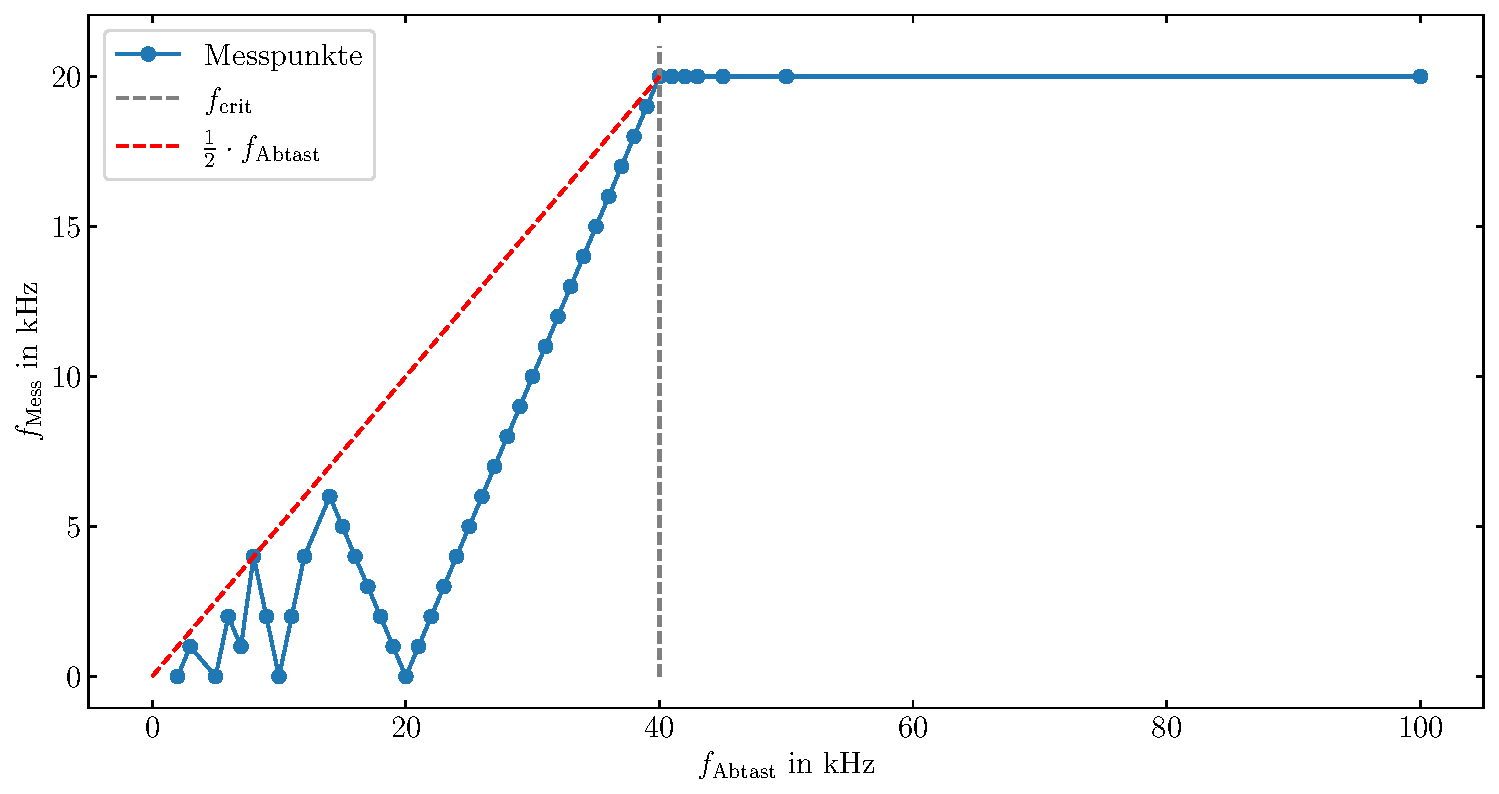
\includegraphics[width=\textwidth]{Paul/42a1.pdf}
    \caption{Variation der Abtastrate gegen die gemessene Frequenz, bei konstanter Generatorfrequenz von 20 kHz.}
    \label{fig:42a1}
\end{figure}

In Abbildung \ref{fig:42a1} ist deutlich zu erkennen, dass für die Abtastfrequenz $f_{Abtast} > f_{crit}$ die Frequenz korrekt gemessen wird. Bei unterschreiten der kritischen Frequenz fällt die gemessene Frequenz jedoch unter den eigentlichen Wert, bis $f = f_{Abtast}$. Wenn die Abtastfrequenz gleich der Generatorfrequenz ist, wird eine Frequenz von 0 Hz gemessen, also ein konstantes Signal. Das ist logisch, da der Detektor immer den gleichen Punkt der Signalabfolge misst und dies somit als konstantes Signal wahrnimmt. Dies tritt nicht nur für $f = f_{Abtast}$ auf, sondern immer dann wenn $f_{Abtast} = n \cdot f$ mit $ n= 1,2,3...$. Aus diesem Grund entsteht vor der kritischen Frequenz ein sägezahnähnliches Muster.

\newpage
In der zweiten Messreihe wurde nun die Abtastrate ($f_{Abtast} = 20$\,kHz) konstant gehalten und die Frequenz des Generators wurde variiert, welche wiederum gegen die gemessene Frequenz aufgetragen wurde. Für die kritische Frequenz gilt nun:
\begin{align}
    f_{crit} = \frac{1}{2} f_{Abtast}
\end{align}
\begin{figure}[h]
    \centering
    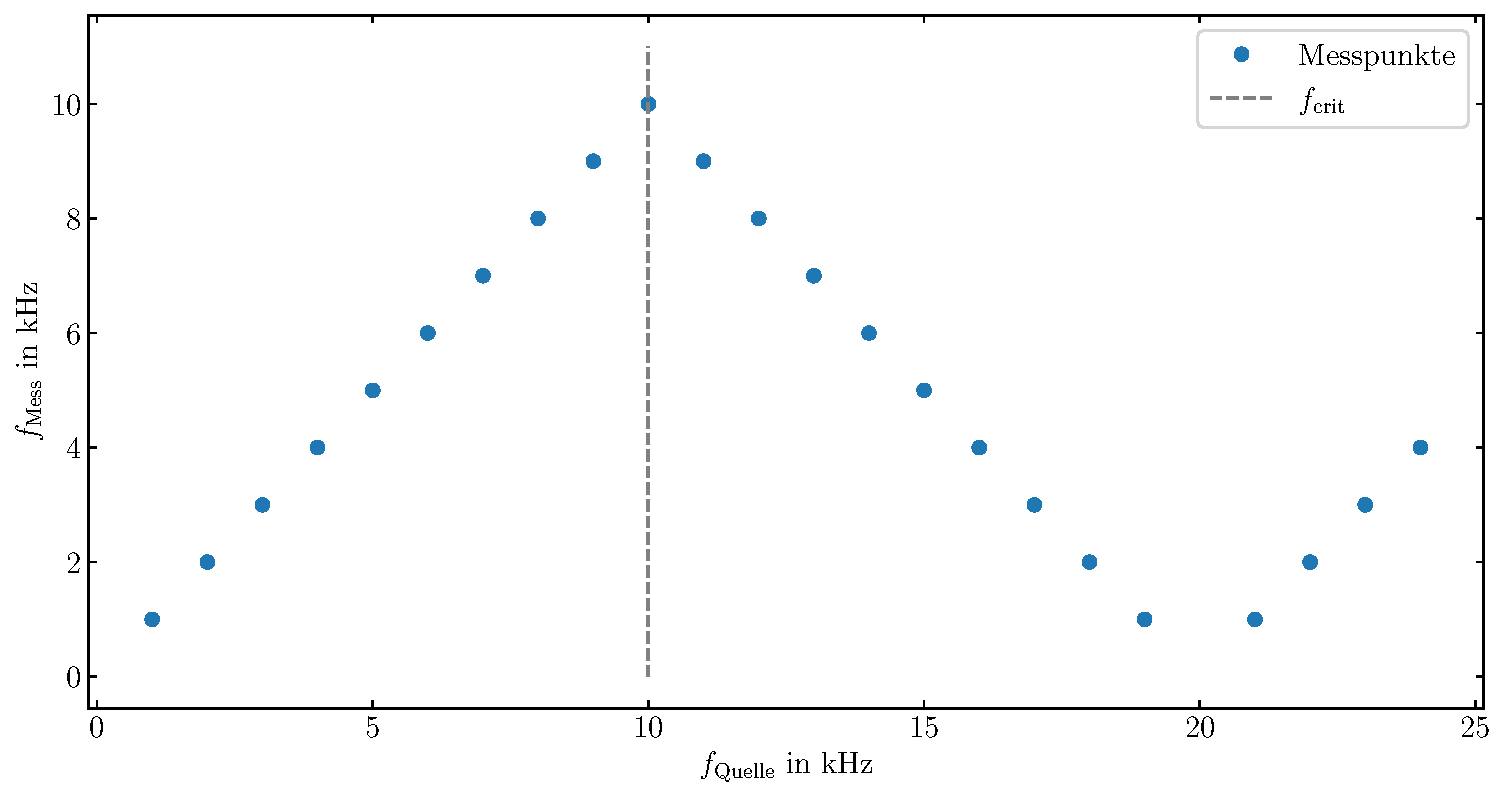
\includegraphics[width=\textwidth]{Paul/42a2.pdf}
    \caption{Variation der Generatorfrequenz gegen die gemessene Frequenz, bei konstanter Abtastfrequenz.}
    \label{fig:42a2}
\end{figure}
In Abbildung \ref{fig:42a2} ist wieder deutlich zu sehen, dass für $f_{Quelle} < f_{crit}$ die Frequenz richtig gemessen wird. Ist dies jedoch nicht mehr der Fall, so tritt analog zu oben wieder ein Sägezahnmuster auf.


\newpage
Des Weiteren wurde das Fourierspektrum eines Dreieckssignal ($f = 3$\,kHz), mit einer Abtastfrequenz von $f_s = 7$\,kHz, aufgenommen.
\begin{figure}[h]
    \centering
    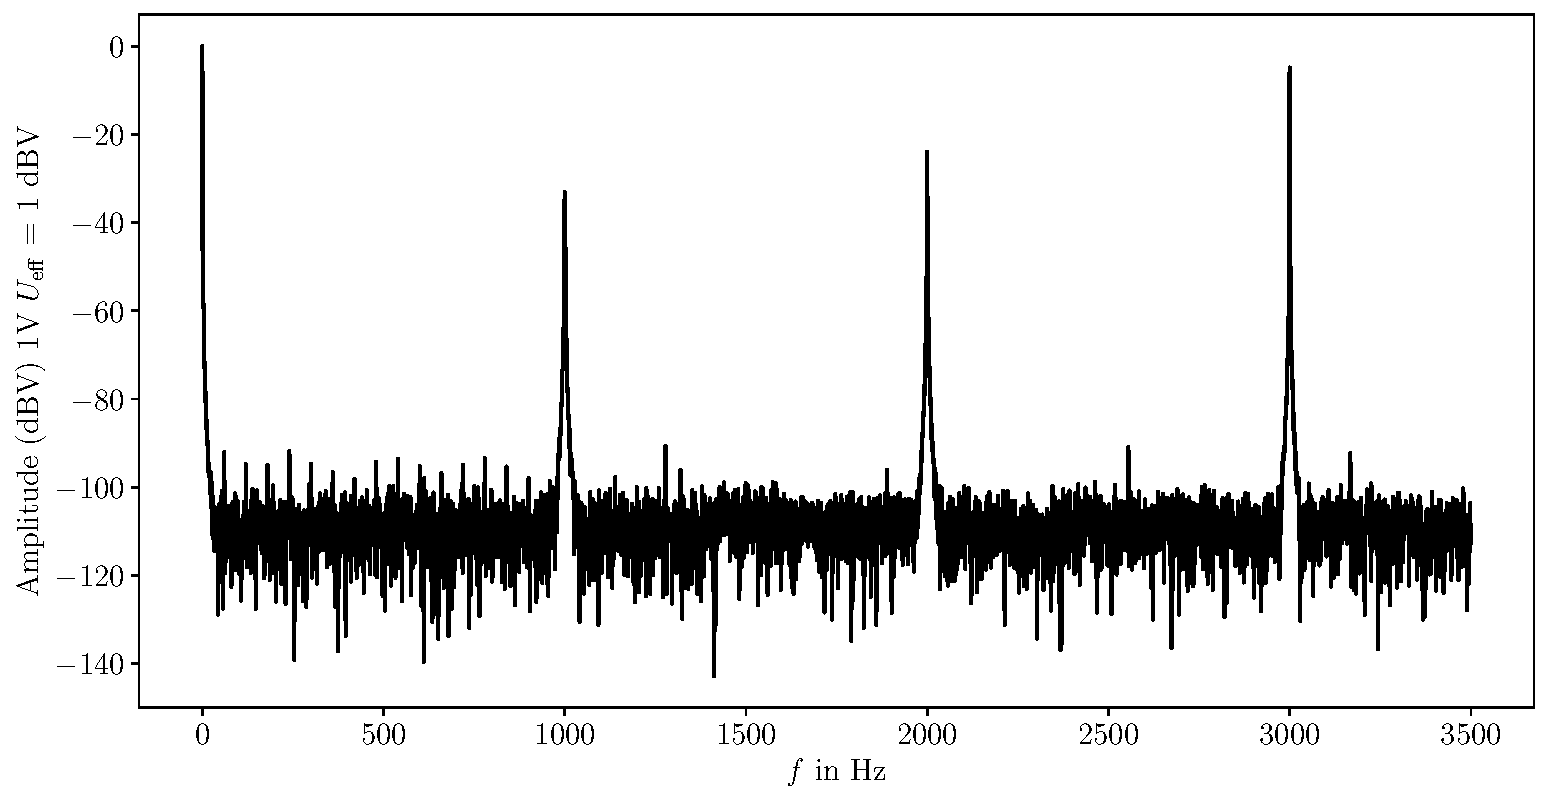
\includegraphics[width=\textwidth]{Paul/42b-fs7kHz.pdf}
    \caption{Fourierspektrum eines Dreieckssignal ($f = 3$\,kHz), $f_s = 7$\,kHz.}
    \label{fig:42a3}
\end{figure}

In Abbildung \ref{fig:42a3} ist der Effekt des Aliasing zu erkennen, das heißt der Detektor kann nicht unterscheiden, welche die richtig gemessene Frequenz ist und was die Aliase (falsche zugeordnete Messwerte) der eigentlichen Frequenz sind. Da die Generatorfrequenz bekannt ist, ist ebenfalls bekannt, dass die richtige Frequenz $f=3$\,kHz ist und die Peaks bei $f_1=1$\,kHz und $f_2=2$\,kHz die Aliase dieser sind. Hat man dieses wissen jedoch nicht, kann dies jedoch zu nicht unerheblichen Messfehlern führen. Um Aliasing zu vermeiden, sollte eine höhere Abtastfrequenz verwendet werden.\\

%TODO #42
Erklärung d. Peaks --> Umklappprozesse